%!TEX root = ../rsra.tex

\chapter{Introduction}
\section{Why reliability is so important?}

\begin{figure}[!htp]
    \centering
    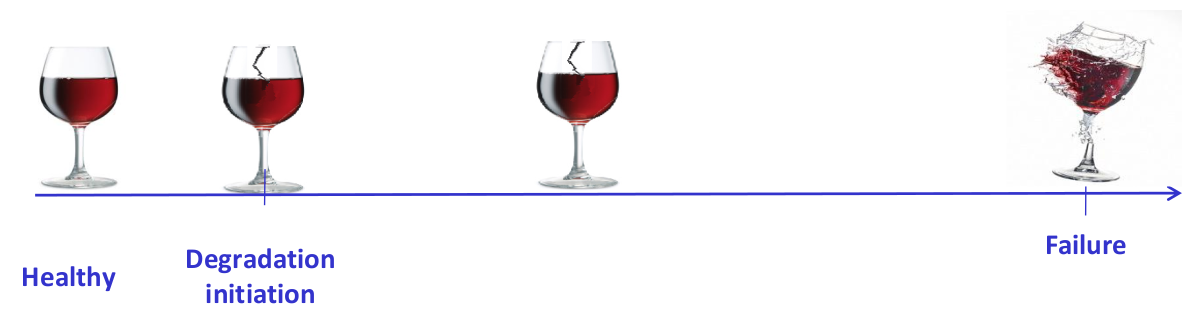
\includegraphics[width=.85\textwidth]{evolution_to_failure}
    \caption{Evolution to failure...}
\end{figure}

A component, even if very well designed, built with durable materials from the
best manufacturer in the world, will eventually start degrading $\to$
\emph{onset of a degradation process}.

Degradation won't stop and, without proper countermeasures, the component will
fail at a given point. We cannot ignore it!

\section{Examples of Degradation}
\subsection{Creep of turbine blades}

Creep failure is one of the most important failure modes of turbine blade. Creep
is the progressive time-dependent inelastic deformation under mechanical load
and high temperature.

The deformation may become so large that a turbine blade could cause the blade
to contact the casing, resulting in the failure of the blade.

\begin{figure}[!htp]
    \centering
    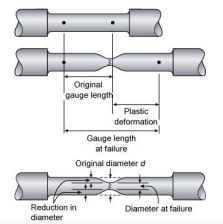
\includegraphics[width=.3\textwidth]{creeping_1}
    \caption{Cree of turbine blades}
\end{figure}

The rupture of one of multiple blades renders the turbine unbalanced, leading to
the failure of the turbine bearings. The shock from such an accident can produce
projectiles with a range in the order of a hundred metres.

\begin{figure}[!htp]
    \centering
    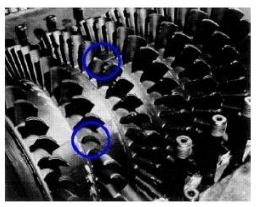
\includegraphics[width=.5\textwidth]{creeping_2}
    \caption{Turbine with blades damaged by creeping}
\end{figure}

\subsection{Erosion of choke valves}
The \emph{choke valve} is a type of control valve, mostly used in oil and gas
production wells to control the flow of well fluids being produced.

Choke valves allow fluid flow through a very small opening, designed to kill the
reservoir pressure while regulating the well production. The reservoir fluids
can contain sand particles. Hence the choke valves are usually designed to
handle an erosive service.

\begin{figure}[!htp]
    \centering
    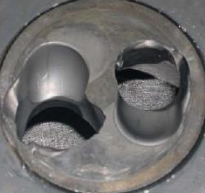
\includegraphics[width=.3\textwidth]{eroded_valve}
    \caption{Erosion of a choke valve}
\end{figure}

Replacing a valve hundreds of metres under the sea level is a challenging task
and should happen \emph{as infrequently as possible}.

\subsection{Crack propagation}
\begin{figure}[!htp]
    \centering
    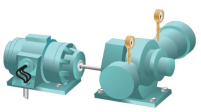
\includegraphics[width=.3\textwidth]{industrial_machine}
    \caption{Pump driven by an electric motor}
\end{figure}

Bearings can suffer crack propagation, leading to possible catastrophic
consequences in an engine.

\begin{figure}[!htp]
    \centering
    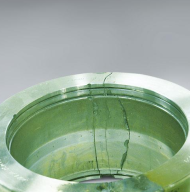
\includegraphics[width=.3\textwidth]{crack_propagation}
    \caption{Crack propagation in bearing}
\end{figure}

\section{Examples of Failure}
\subsection{From the Nuclear industry: the Devis-Besse accident}

In March 2002, plant staff discovered that the borated water that serves as the
reactor coolant had leaked from cracked control rod drive mechanisms directly
above the reactor and eaten through more than 150 mm of the carbon steel reactor
pressure vessel head (Fig.~\ref{fig:devis_besse}) over an area roughly the
size of a football.

\begin{figure}[!htp]
    \centering
    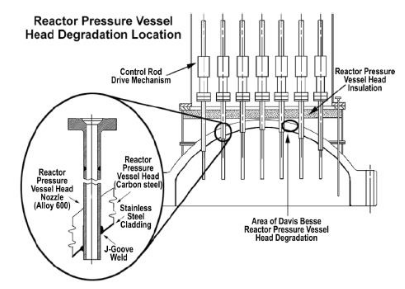
\includegraphics[width=.5\textwidth]{devis_besse}
    \caption{Reactor pressure vessel head}
    \label{fig:devis_besse}
\end{figure}

This significant reactor head wastage on the exterior of the reactor vessel head
left only 9.5 mm of stainless steel cladding holding back the high-pressure
(14.6 MPa) reactor coolant.

Consequences:
\begin{itemize}
    \item 600 M\$ spent for a new lid;
    \item the NRC kept Davis–Besse shut down until March 2004, so that
    FirstEnergy was able to perform all the necessary maintenance for safe
    operations (2 years).
\end{itemize}

Possible consequences in case of failure (rupture):
\begin{itemize}
    \item \emph{Loss Of Coolant Accident} that triggers emergency safety procedures to protect from core damage or meltdown. However, the jet of reactor coolant might have damaged adjacent control rod drive mechanisms, hampering or preventing reactor shut-down and leading to a core meltdown.
\end{itemize}

\subsection{From the Oil and Gas industry: Deepwater Horizon oil spill}
\begin{figure}[!htp]
    \centering
    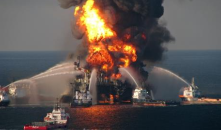
\includegraphics[width=.3\textwidth]{deepwater_horizon}
    \caption{Explosion of the platform Deepwater Horizon}
\end{figure}

\begin{figure}[!htp]
    \centering
    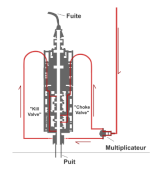
\includegraphics[width=.3\textwidth]{deepwater_horizon_cause}
    \caption{Probable cause: leakage in the oil pumping system}
\end{figure}

\subsection{From the Railway industry: Brétigny-sur-Orge train crash}
\begin{figure}[!htp]
    \centering
    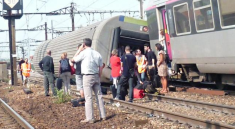
\includegraphics[width=.3\textwidth]{train_crash}
    \caption{TODO}
\end{figure}

\begin{figure}[!htp]
    \centering
    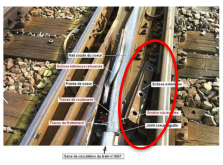
\includegraphics[width=.3\textwidth]{train_crash_detail}
    \caption{TODO}
\end{figure}

\subsection{From Construction industry: Collapse of Morandi Bridge}